\documentclass[aspectratio=169,10pt]{beamer}
\usepackage[T1]{fontenc}
\usepackage[utf8]{inputenc}
\usepackage{tikz}
\usetikzlibrary{shapes.geometric,arrows.meta,positioning,fit,calc}
\usepackage{listings}

% ---------- Theme ----------
\definecolor{navy}{RGB}{20,50,90}
\definecolor{teal}{RGB}{0,128,128}
\definecolor{amber}{RGB}{240,170,40}
\definecolor{soft}{RGB}{230,240,248}
\definecolor{softgreen}{RGB}{225,245,232}
\definecolor{softred}{RGB}{250,228,228}
\setbeamercolor{frametitle}{bg=navy,fg=white}
\setbeamercolor{title}{fg=navy}
\setbeamercolor{structure}{fg=teal}
\setbeamertemplate{navigation symbols}{}
\setbeamertemplate{footline}{\hfill\insertframenumber\hspace{1em}\vspace{4pt}}
\setbeamertemplate{itemize item}{\color{teal}$\blacktriangleright$}

% ---------- Code listing style ----------
\lstset{
  language=Python,
  basicstyle=\ttfamily\small,
  keywordstyle=\color{navy}\bfseries,
  commentstyle=\color{teal},
  stringstyle=\color{red!60!black},
  showstringspaces=false,
  breaklines=true,
  columns=flexible,
  frame=single,
  rulecolor=\color{navy!40},
  backgroundcolor=\color{soft},
  xleftmargin=2pt,
  aboveskip=2pt,belowskip=2pt
}

% ---------- Diagram styles ----------
\tikzset{
  box/.style={rectangle,rounded corners=4pt,draw=navy,fill=soft,thick,align=center,
              minimum height=1.0cm,text width=2.2cm,font=\footnotesize,inner sep=3pt},
  store/.style={cylinder,shape border rotate=90,aspect=0.25,draw=navy,fill=softgreen,
              thick,align=center,minimum height=1.3cm,text width=2cm,font=\footnotesize,inner sep=2pt},
  dec/.style={diamond,draw=navy,fill=amber!40,thick,align=center,
              font=\scriptsize,text width=2.4cm,inner sep=0pt,minimum width=3.6cm,minimum height=1.5cm},
  out/.style={rectangle,rounded corners=4pt,draw=teal,fill=teal!20,thick,align=center,
              minimum height=1.0cm,text width=2.4cm,font=\footnotesize,inner sep=3pt},
  arr/.style={-{Stealth[length=2.5mm]},thick,navy},
  lbl/.style={font=\scriptsize,fill=white,inner sep=1pt}
}

\title{RAG Model for NCERT Science (Class 6--12)}
\subtitle{Understanding Chunking for Retrieval-Augmented Generation}
\author{\footnotesize Project Mentor : Dr. Ashish Kumar Sahu\\[6pt]
  Members :\\ Sarthak Mittal\\ Chandan Gupta\\ Aryan Chilkewar\\ Agrim Salhotra}
\date{}

\begin{document}

% 1 ---------------------------------------------------
\begin{frame}
  \titlepage
\end{frame}

% 2 ---------------------------------------------------
\begin{frame}[t]{Topics Covered in This Lecture}
\begin{itemize}
  \item What Retrieval-Augmented Generation (RAG) is and why it is used.
  \item What chunking is, and why the way we cut a document matters.
  \item Six common chunking strategies, with diagrams, code, advantages and disadvantages.
  \item How to choose a strategy for a textbook such as NCERT Science.
  \item Research findings on chunking, explained in simple terms.
\end{itemize}
\end{frame}

% 3 ---------------------------------------------------
\begin{frame}[t]{Why Not Just Ask the LLM Directly?}
\small
A Large Language Model (LLM) answers from what it learned during training. For school or university content, this causes two problems.
\begin{itemize}
  \item \textbf{Hallucination:} the model can give a confident answer that is wrong.
  \item \textbf{Off-syllabus answers:} the model may use advanced explanations that do not match the textbook.
\end{itemize}
\vspace{14pt}
\begin{center}
\begin{tikzpicture}
  \node[box,text width=2.6cm] (q) at (-3.6,0) {Student question};
  \node[box,fill=softred,text width=2.8cm] (l) at (0,0) {LLM alone (no textbook)};
  \node[out,fill=softred,draw=red!60!black,text width=3.2cm] (a) at (3.9,0) {Possibly wrong or off-syllabus answer};
  \draw[arr] (q.east)--(l.west);
  \draw[arr] (l.east)--(a.west);
\end{tikzpicture}
\end{center}
\end{frame}

% 4 ---------------------------------------------------
\begin{frame}[t]{Retrieval-Augmented Generation (RAG)}
\small
RAG first \emph{finds} the relevant text in a document collection. Then it gives that text to the LLM, which answers from it.
\vspace{14pt}
\begin{center}
\begin{tikzpicture}
  % top row: building the database
  \node[box] (doc) at (0,0) {Textbook (PDF)};
  \node[box,fill=amber!30] (chunk) at (2.9,0) {1. Chunking};
  \node[box] (emb) at (5.8,0) {2. Embedding (number vectors)};
  \node[store] (db) at (8.7,0) {Vector database};
  % bottom row: answering a question
  \node[box] (q) at (0,-2.4) {Student question};
  \node[box,fill=amber!30] (qe) at (2.9,-2.4) {Embed the question};
  \node[box,fill=amber!30] (top) at (5.8,-2.4) {3. Find top-K similar chunks};
  \node[box,fill=amber!30] (llm) at (8.7,-2.4) {4. LLM writes the answer};
  \node[out] (ans) at (8.7,-4.6) {Answer with source};
  \draw[arr] (doc)--(chunk); \draw[arr] (chunk)--(emb); \draw[arr] (emb)--(db);
  \draw[arr] (q)--(qe); \draw[arr] (qe)--(top);
  \draw[arr] (db.south) -- (8.7,-1.2) -- (5.8,-1.2) -- (top.north);
  \draw[arr] (top)--(llm); \draw[arr] (llm)--(ans);
  \node[font=\scriptsize,anchor=west] at (-0.9,-3.4) {Both the textbook and the question use the same embedding model.};
\end{tikzpicture}
\end{center}
\end{frame}

% 5 ---------------------------------------------------
\begin{frame}[t]{Key Words in Plain Language}
\small
\begin{itemize}
  \item \textbf{Token:} a small piece of text that a model reads, often a word or part of a word.
  \item \textbf{Chunk:} one piece of a document that we store and search as a single unit.
  \item \textbf{Embedding:} a list of numbers that represents the meaning of a piece of text.
  \item \textbf{Vector:} the same as an embedding. It is a point in a space with many dimensions.
  \item \textbf{Similarity:} how close two vectors are. Close vectors mean similar meaning.
  \item \textbf{Retrieval:} finding the chunks most similar to the question.
  \item \textbf{Top-K:} the K best-matching chunks. For example, top-5 means the five best.
\end{itemize}
\end{frame}

% 6 ---------------------------------------------------
\begin{frame}[t]{An Analogy: Library Cards}
\small
Think of a textbook as a long scroll. Chunking cuts the scroll into cards. Each card gets a label, so a search can find the right card quickly.
\vspace{14pt}
\begin{center}
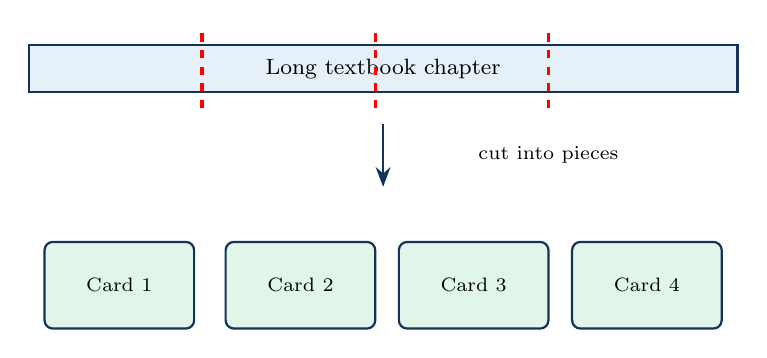
\begin{tikzpicture}
  \draw[navy,thick,fill=soft] (0,3.0) rectangle (9,3.6);
  \node[font=\footnotesize] at (4.5,3.3) {Long textbook chapter};
  \draw[very thick,red,dashed] (2.2,2.8) -- (2.2,3.8);
  \draw[very thick,red,dashed] (4.4,2.8) -- (4.4,3.8);
  \draw[very thick,red,dashed] (6.6,2.8) -- (6.6,3.8);
  \draw[arr] (4.5,2.6) -- (4.5,1.8);
  \node[font=\scriptsize] at (6.6,2.2) {cut into pieces};
  \foreach \x/\n in {0.2/1,2.5/2,4.7/3,6.9/4}{
    \draw[navy,thick,rounded corners=3pt,fill=softgreen] (\x,0) rectangle (\x+1.9,1.1);
    \node[font=\scriptsize] at (\x+0.95,0.55) {Card \n};
  }
\end{tikzpicture}
\end{center}
\vspace{4pt}
\small
Small, labelled cards are easier to search than one very long scroll.
\end{frame}

% 7 ---------------------------------------------------
\begin{frame}[t]{What Is Chunking?}
\small
Chunking means splitting a long document into smaller pieces before we create embeddings and store them.
\vspace{14pt}
\begin{center}
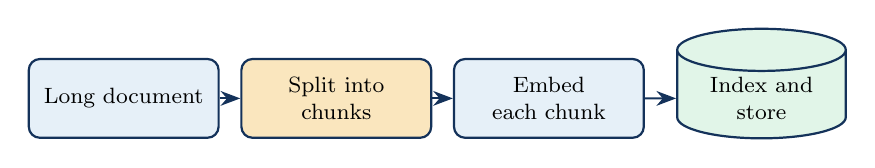
\begin{tikzpicture}
  \node[box] (a) at (0,0) {Long document};
  \node[box,fill=amber!30] (b) at (2.7,0) {Split into chunks};
  \node[box] (c) at (5.4,0) {Embed each chunk};
  \node[store] (d) at (8.1,0) {Index and store};
  \draw[arr] (a)--(b); \draw[arr] (b)--(c); \draw[arr] (c)--(d);
\end{tikzpicture}
\end{center}
\vspace{14pt}
\begin{itemize}
  \item A chunk that is too large may mix several topics, so its embedding becomes vague.
  \item A chunk that is too small may lose the context needed to understand it.
\end{itemize}
\end{frame}

% 8 ---------------------------------------------------
\begin{frame}[t]{Why Chunk Size Matters}
\small
The same sentence can mean different things depending on what surrounds it.
\vspace{14pt}
\begin{center}
\begin{tikzpicture}
  \node[box,text width=6.5cm,fill=softred] (s) at (0,0) {``It takes place mainly in the leaves.''};
  \node[out,text width=6.5cm] (g) at (0,-2.2) {Good chunk: it also contains ``Photosynthesis is the process\ldots'', so ``It'' is clear.};
  \node[box,text width=6.5cm,fill=softred] (b) at (0,-4.4) {Too small: the chunk is only this sentence, so ``It'' is unclear.};
  \draw[arr] (s)--(g);
\end{tikzpicture}
\end{center}
\end{frame}

% 9 ---------------------------------------------------
\begin{frame}[t]{Running Example Used in This Lecture}
\small
This short paragraph is used on every strategy slide, so the methods can be compared on the same text.
\vspace{14pt}
\begin{center}
\fcolorbox{navy}{soft}{\parbox{0.9\textwidth}{\normalsize
Photosynthesis is the process by which green plants prepare food. It takes place mainly in the leaves. Chlorophyll in the chloroplasts absorbs sunlight. Carbon dioxide enters through stomata, and water is absorbed by the roots. The overall equation is $6\mathrm{CO_2} + 6\mathrm{H_2O} \rightarrow \mathrm{C_6H_{12}O_6} + 6\mathrm{O_2}$.}}
\end{center}
\end{frame}

% 10 --------------------------------------------------
\begin{frame}[t]{Six Chunking Strategies at a Glance}
\small
Strategies are listed from simplest to most complex. More complex methods usually cost more to build and run.
\vspace{18pt}
\begin{center}
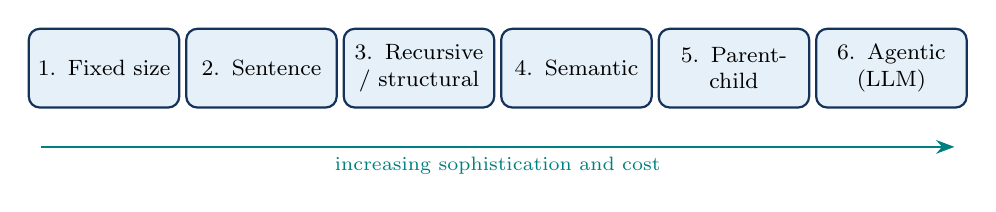
\begin{tikzpicture}
  \node[box,text width=1.7cm] (s1) at (0,0) {1. Fixed size};
  \node[box,text width=1.7cm] (s2) at (2.0,0) {2. Sentence};
  \node[box,text width=1.7cm] (s3) at (4.0,0) {3. Recursive / structural};
  \node[box,text width=1.7cm] (s4) at (6.0,0) {4. Semantic};
  \node[box,text width=1.7cm] (s5) at (8.0,0) {5. Parent-child};
  \node[box,text width=1.7cm] (s6) at (10.0,0) {6. Agentic (LLM)};
  \draw[thick,teal,-{Stealth}] (-0.8,-1.0) -- node[below,font=\scriptsize]{increasing sophistication and cost} (10.8,-1.0);
\end{tikzpicture}
\end{center}
\end{frame}

% 11 --------------------------------------------------
\begin{frame}[t]{Strategy 1: Fixed-Size Chunking (Idea)}
\small
Cut the text every $N$ characters or tokens. An optional overlap repeats a few characters at the start of the next chunk.
\vspace{14pt}
\begin{center}
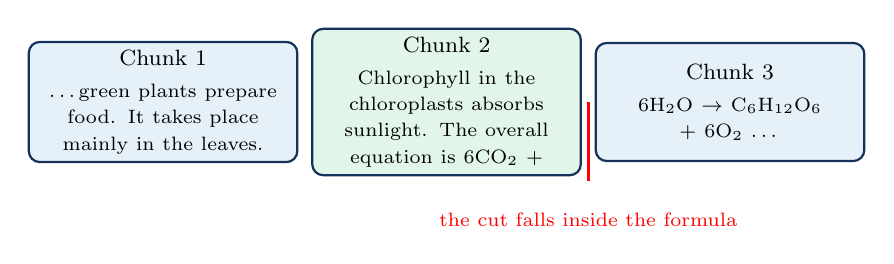
\begin{tikzpicture}
  \node[box,text width=3.2cm,minimum height=1.5cm] (c1) at (0,0) {Chunk 1\\[2pt]\scriptsize \ldots green plants prepare food. It takes place mainly in the leaves.};
  \node[box,text width=3.2cm,minimum height=1.5cm,fill=softgreen] (c2) at (3.6,0) {Chunk 2\\[2pt]\scriptsize Chlorophyll in the chloroplasts absorbs sunlight. The overall equation is 6CO$_2$ +};
  \node[box,text width=3.2cm,minimum height=1.5cm] (c3) at (7.2,0) {Chunk 3\\[2pt]\scriptsize 6H$_2$O $\rightarrow$ C$_6$H$_{12}$O$_6$ + 6O$_2$ \ldots};
  \draw[very thick,red] (5.4,-1.0) -- (5.4,0.0);
  \node[font=\scriptsize,red] at (5.4,-1.5) {the cut falls inside the formula};
\end{tikzpicture}
\end{center}
\end{frame}

% 12 --------------------------------------------------
\begin{frame}[t,fragile]{Strategy 1: Fixed-Size Chunking (Code and Trade-offs)}
\small
\begin{lstlisting}
def fixed_chunks(text, size=60, overlap=0):
    chunks = []
    start = 0
    while start < len(text):
        chunks.append(text[start:start + size])
        start += size - overlap
    return chunks
\end{lstlisting}
\vspace{6pt}
\begin{columns}[T]
\column{0.5\textwidth}
\textbf{Advantages}
\begin{itemize}
  \item Very simple to write and fast to run.
  \item Every chunk has about the same size, which makes storage easy.
\end{itemize}
\column{0.5\textwidth}
\textbf{Disadvantages}
\begin{itemize}
  \item Ignores meaning, so it can cut sentences, definitions and equations.
  \item The size must be tuned, and the best value depends on the document.
\end{itemize}
\end{columns}
\end{frame}

% 13 --------------------------------------------------
\begin{frame}[t]{Strategy 2: Sentence-Based Chunking (Idea)}
\small
Split the text at sentence endings, then group one or a few whole sentences into each chunk. No sentence is cut in half.
\vspace{14pt}
\begin{center}
\begin{tikzpicture}
  \node[box,text width=2.4cm] (s1) at (0,0) {Photosynthesis is the process\ldots};
  \node[box,text width=2.4cm] (s2) at (2.9,0) {It takes place mainly in the leaves.};
  \node[box,text width=2.4cm] (s3) at (5.8,0) {Chlorophyll absorbs sunlight.};
  \node[out] (c) at (2.9,-2.4) {One chunk per sentence, or per small group};
  \draw[arr] (s2)--(c);
\end{tikzpicture}
\end{center}
\end{frame}

% 14 --------------------------------------------------
\begin{frame}[t,fragile]{Strategy 2: Sentence-Based Chunking (Code and Trade-offs)}
\small
\begin{lstlisting}
import re

def sentence_chunks(text):
    parts = re.split(r'(?<=[.!?])\s+', text)
    return [p.strip() for p in parts if p.strip()]
\end{lstlisting}
\vspace{6pt}
\begin{columns}[T]
\column{0.5\textwidth}
\textbf{Advantages}
\begin{itemize}
  \item Never cuts a sentence, so each chunk reads naturally.
  \item Cheap to compute, and no model is needed.
\end{itemize}
\column{0.5\textwidth}
\textbf{Disadvantages}
\begin{itemize}
  \item One sentence can lack context. ``It takes place\ldots'' does not say what ``It'' is.
  \item Simple rules fail on abbreviations such as ``e.g.'' and on equations that contain full stops.
\end{itemize}
\end{columns}
\end{frame}

% 15 --------------------------------------------------
\begin{frame}[t]{Strategy 3: Recursive / Structural Chunking (Idea)}
\small
Split by the largest structure first (sections), then by smaller units (paragraphs, then sentences). Keep going until every chunk fits the size limit.
\vspace{14pt}
\begin{center}
\begin{tikzpicture}
  \node[box,text width=3.4cm] (a) at (0,0) {Chapter or section};
  \node[box,text width=3.4cm] (b) at (0,-1.9) {Paragraphs (too big? split further)};
  \node[box,text width=3.4cm] (c) at (0,-3.8) {Sentences (too big? split further)};
  \node[out,text width=3cm] (d) at (6.0,-1.9) {Chunks that fit the size limit};
  \draw[arr] (a)--(b); \draw[arr] (b)--(c);
  \draw[arr] (b.east)--(d.west);
  \draw[arr] (c.east) -- (3.0,-3.8) -- (3.0,-1.9) -- (b.east);
\end{tikzpicture}
\end{center}
\end{frame}

% 16 --------------------------------------------------
\begin{frame}[t,fragile]{Strategy 3: Recursive / Structural Chunking (Code and Trade-offs)}
\small
\begin{lstlisting}
from langchain_text_splitters import RecursiveCharacterTextSplitter

splitter = RecursiveCharacterTextSplitter(
    chunk_size=500, chunk_overlap=50,
    separators=["\n\n", "\n", ". ", " ", ""])
chunks = splitter.split_text(chapter_text)
\end{lstlisting}
\vspace{6pt}
\begin{columns}[T]
\column{0.5\textwidth}
\textbf{Advantages}
\begin{itemize}
  \item Follows the document's own structure, so a whole topic can stay together.
  \item Works well for textbooks that have clear headings.
\end{itemize}
\column{0.5\textwidth}
\textbf{Disadvantages}
\begin{itemize}
  \item Chunk sizes vary, and very long sections still need splitting.
  \item Depends on clean text. Poorly extracted headings lead to poor chunks.
\end{itemize}
\end{columns}
\end{frame}

% 17 --------------------------------------------------
\begin{frame}[t]{Strategy 4: Semantic Chunking (Idea)}
\small
Measure how similar each sentence is to the next one. Start a new chunk where similarity drops sharply, because the topic has changed.
\vspace{14pt}
\begin{center}
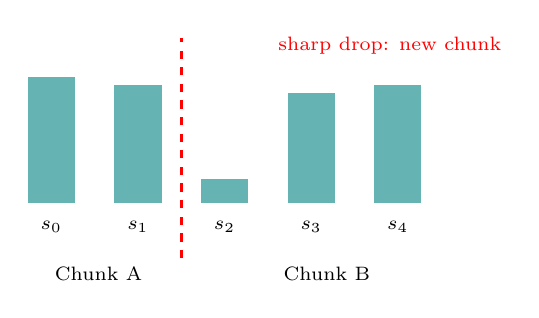
\begin{tikzpicture}
  \foreach \i/\h in {0/1.6,1/1.5,2/0.3,3/1.4,4/1.5}{
    \fill[teal!60] (\i*1.1,0) rectangle (\i*1.1+0.6,\h);
    \node[font=\scriptsize] at (\i*1.1+0.3,-0.3) {$s_{\i}$};
  }
  \draw[very thick,red,dashed] (1.95,-0.7) -- (1.95,2.1);
  \node[font=\scriptsize,red] at (4.6,2.0) {sharp drop: new chunk};
  \node[font=\scriptsize] at (0.9,-0.9) {Chunk A};
  \node[font=\scriptsize] at (3.8,-0.9) {Chunk B};
\end{tikzpicture}
\end{center}
\vspace{4pt}
\small
Bar height shows how similar a sentence is to the one before it (illustrative values).
\end{frame}

% 18 --------------------------------------------------
\begin{frame}[t,fragile]{Strategy 4: Semantic Chunking (Code and Trade-offs)}
\small
\lstset{basicstyle=\ttfamily\footnotesize}
\begin{lstlisting}
from sentence_transformers import SentenceTransformer
import numpy as np

model = SentenceTransformer("all-MiniLM-L6-v2")
emb = model.encode(sentences, normalize_embeddings=True)

chunks, current = [], [sentences[0]]
for i in range(1, len(sentences)):
    sim = float(np.dot(emb[i-1], emb[i]))
    if sim < 0.5:                  # threshold: a tuning choice
        chunks.append(" ".join(current))
        current = []
    current.append(sentences[i])
chunks.append(" ".join(current))
\end{lstlisting}
\vspace{4pt}
\begin{columns}[T]
\column{0.5\textwidth}
\textbf{Advantages}
\begin{itemize}
  \item Follows real topic changes, such as a move from plant cells to animal cells.
\end{itemize}
\column{0.5\textwidth}
\textbf{Disadvantages}
\begin{itemize}
  \item Needs an embedding for every sentence, which costs time during ingestion.
  \item The threshold changes the result, so it must be tested on your own data.
\end{itemize}
\end{columns}
\end{frame}

% 19 --------------------------------------------------
\begin{frame}[t]{Strategy 5: Parent-Child Chunking (Idea)}
\small
Search with small \emph{child} chunks, which are precise. Send the larger \emph{parent} chunk to the LLM, which gives more context.
\vspace{14pt}
\begin{center}
\begin{tikzpicture}
  \node[store,text width=2.2cm] (v) at (0,0) {Child chunks (search here)};
  \node[store,text width=2.2cm,fill=amber!30] (d) at (5.2,0) {Parent chunks (full paragraph)};
  \node[box,text width=3.0cm] (m) at (0,-2.8) {Child matched: ``Chlorophyll absorbs sunlight.''};
  \node[out,text width=3.0cm] (l) at (5.2,-2.8) {Parent sent to the LLM};
  \draw[arr] (v)--(m) node[lbl,midway,left=2pt]{search};
  \draw[arr] (m)--(l) node[lbl,midway,below=2pt]{link to parent};
  \draw[arr] (d)--(l);
\end{tikzpicture}
\end{center}
\end{frame}

% 20 --------------------------------------------------
\begin{frame}[t,fragile]{Strategy 5: Parent-Child Chunking (Code and Trade-offs)}
\small
\begin{lstlisting}
parents = {"P1": "Photosynthesis is the process ... 6O2."}
children = [
    {"text": "Chlorophyll absorbs sunlight.", "parent": "P1"},
    {"text": "The overall equation is 6CO2 + 6H2O -> C6H12O6 + 6O2.", "parent": "P1"},
]

def answer_context(query):
    best = search_children(query)      # vector search over child texts
    return parents[best["parent"]]     # send the whole parent to the LLM
\end{lstlisting}
\vspace{6pt}
\begin{columns}[T]
\column{0.5\textwidth}
\textbf{Advantages}
\begin{itemize}
  \item Precise search and enough context for the answer.
  \item Useful when a formula is short but its explanation is in the paragraph around it.
\end{itemize}
\column{0.5\textwidth}
\textbf{Disadvantages}
\begin{itemize}
  \item Needs two stores: a vector index and a document store.
  \item More code to write and maintain.
\end{itemize}
\end{columns}
\end{frame}

% 21 --------------------------------------------------
\begin{frame}[t]{Strategy 6: Agentic / LLM-Assisted (Propositional) Chunking}
\small
An LLM reads each paragraph and rewrites it as short, standalone facts. Each fact becomes one chunk.
\vspace{14pt}
\begin{center}
\begin{tikzpicture}
  \node[box] (p) at (0,0) {Complex paragraph};
  \node[box,fill=amber!30] (l) at (3.0,0) {LLM};
  \node[out,text width=3.4cm] (f1) at (6.6,1.2) {Fact 1: Chlorophyll absorbs sunlight.};
  \node[out,text width=3.4cm] (f2) at (6.6,0) {Fact 2: Photosynthesis makes food.};
  \node[out,text width=3.4cm] (f3) at (6.6,-1.2) {Fact 3: Oxygen is released.};
  \draw[arr] (p)--(l);
  \draw[arr] (l.east) -- (f1.west);
  \draw[arr] (l.east) -- (f2.west);
  \draw[arr] (l.east) -- (f3.west);
\end{tikzpicture}
\end{center}
\vspace{10pt}
\begin{columns}[T]
\column{0.5\textwidth}
\textbf{Advantages}
\begin{itemize}
  \item Each chunk holds one clear fact, which suits short factual questions.
\end{itemize}
\column{0.5\textwidth}
\textbf{Disadvantages}
\begin{itemize}
  \item Slow and costly, because an LLM must process the whole book before indexing.
  \item The LLM may change the meaning, so errors are stored in the index.
\end{itemize}
\end{columns}
\end{frame}

% 22 --------------------------------------------------
\begin{frame}[t]{Trade-off: Small Chunks vs Large Chunks}
\small
Smaller chunks tend to be more precise. Larger chunks tend to cover more of the answer.
\vspace{10pt}
\begin{center}
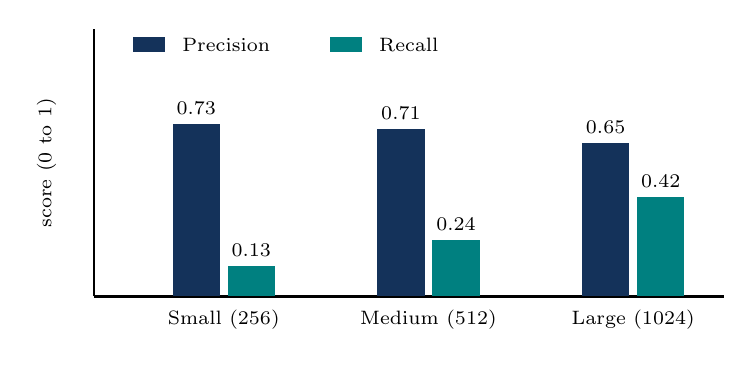
\begin{tikzpicture}
  \draw[thick] (0,0) -- (8,0); \draw[thick] (0,0) -- (0,3.4);
  \node[font=\scriptsize,rotate=90] at (-0.6,1.7) {score (0 to 1)};
  \foreach \x/\p/\r/\lab in {1/0.73/0.13/Small (256),3.6/0.71/0.24/Medium (512),6.2/0.65/0.42/Large (1024)}{
    \fill[navy] (\x,0) rectangle (\x+0.6,\p*3);
    \fill[teal] (\x+0.7,0) rectangle (\x+1.3,\r*3);
    \node[font=\scriptsize] at (\x+0.3,\p*3+0.2) {\p};
    \node[font=\scriptsize] at (\x+1.0,\r*3+0.2) {\r};
    \node[font=\scriptsize] at (\x+0.65,-0.3) {\lab};
  }
  \fill[navy] (0.5,3.1) rectangle (0.9,3.3); \node[font=\scriptsize,anchor=west] at (1.0,3.2) {Precision};
  \fill[teal] (3.0,3.1) rectangle (3.4,3.3); \node[font=\scriptsize,anchor=west] at (3.5,3.2) {Recall};
\end{tikzpicture}
\end{center}
\vspace{6pt}
\small
Precision: how many retrieved chunks are relevant. Recall: how much of the relevant material is retrieved.
\end{frame}

% 23 --------------------------------------------------
\begin{frame}[t]{Overlap: Repeating Some Text Between Chunks}
\small
Overlap copies the last few characters or sentences of one chunk to the start of the next, so a boundary does not lose context.
\vspace{14pt}
\begin{center}
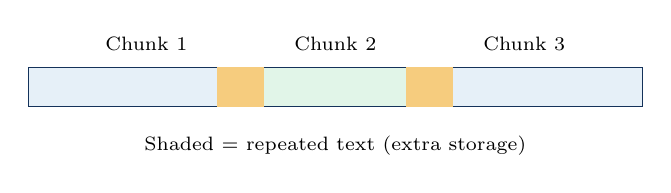
\begin{tikzpicture}
  \fill[soft,draw=navy] (0,1.4) rectangle (3.0,1.9);
  \fill[softgreen,draw=navy] (2.4,1.4) rectangle (5.4,1.9);
  \fill[soft,draw=navy] (4.8,1.4) rectangle (7.8,1.9);
  \fill[amber!60] (2.4,1.4) rectangle (3.0,1.9);
  \fill[amber!60] (4.8,1.4) rectangle (5.4,1.9);
  \node[font=\scriptsize] at (1.5,2.2) {Chunk 1};
  \node[font=\scriptsize] at (3.9,2.2) {Chunk 2};
  \node[font=\scriptsize] at (6.3,2.2) {Chunk 3};
  \node[font=\scriptsize] at (3.9,0.9) {Shaded = repeated text (extra storage)};
\end{tikzpicture}
\end{center}
\vspace{6pt}
\small
In a sentence-based study, 10 to 20 percent overlap gave no measurable gain, while the number of chunks and the index size grew. A common default is no overlap, unless tests show it helps.
\end{frame}

% 24 --------------------------------------------------
\begin{frame}[t]{How Many Chunks to Send to the LLM?}
\small
The retrieved chunks fill a context budget. More context is not always better.
\vspace{10pt}
\begin{center}
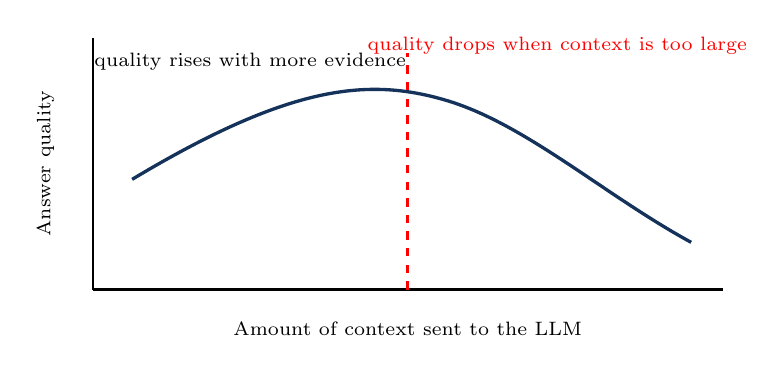
\begin{tikzpicture}
  \draw[thick] (0,0) -- (8,0); \draw[thick] (0,0) -- (0,3.2);
  \node[font=\scriptsize] at (4,-0.5) {Amount of context sent to the LLM};
  \node[font=\scriptsize,rotate=90] at (-0.6,1.6) {Answer quality};
  \draw[very thick,navy] (0.5,1.4) .. controls (2.5,2.6) and (3.5,2.7) .. (4.5,2.4)
     .. controls (5.5,2.1) and (6.5,1.2) .. (7.6,0.6);
  \draw[very thick,red,dashed] (4.0,0) -- (4.0,3.0);
  \node[font=\scriptsize,red] at (5.9,3.1) {quality drops when context is too large};
  \node[font=\scriptsize] at (2.0,2.9) {quality rises with more evidence};
\end{tikzpicture}
\end{center}
\vspace{4pt}
\small
The shape is a general pattern. The exact point where quality drops depends on the model, so test it on your own data.
\end{frame}

% 25 --------------------------------------------------
\begin{frame}[t]{Before Chunking: Extract the Text Correctly}
\small
Chunking can only be as good as the text it receives. Extraction errors from PDFs often matter more than the chunk size.
\vspace{14pt}
\begin{center}
\begin{tikzpicture}
  \node[box,text width=2.2cm] (a) at (-4.6,0) {PDF page};
  \node[box,fill=amber!30,text width=2.6cm] (b) at (-1.4,0) {Extract text, headings, formulas, tables};
  \node[dec,text width=2.2cm,minimum width=3.2cm] (c) at (2.0,0) {Text correct?};
  \node[out,text width=2.0cm] (d) at (5.3,0) {Ready to chunk};
  \node[out,fill=softred,draw=red!60!black,text width=3.0cm] (e) at (2.0,-2.6) {Fix OCR or formula handling};
  \draw[arr] (a)--(b);
  \draw[arr] (b)--(c);
  \draw[arr] (c)--node[lbl,above]{yes}(d);
  \draw[arr] (c)--node[lbl,right]{no}(e);
  \draw[arr] (e.west) -- (-1.4,-2.6) -- (b.south);
\end{tikzpicture}
\end{center}
\vspace{4pt}
\small
Example: if a chemical equation is extracted as ``2H2 O2'' with the arrow missing, no chunking method can recover its meaning.
\end{frame}

% 26 --------------------------------------------------
\begin{frame}[t]{Attach Metadata to Each Chunk}
\small
Metadata is extra information stored with each chunk, such as class, chapter, section and page. The search can filter by these tags before it matches meaning.
\vspace{14pt}
\begin{center}
\begin{tikzpicture}
  \node[box,text width=3.2cm] (q) at (0,0) {Question: ``Explain chlorophyll'' (Class 8, Chapter 6)};
  \node[store,text width=3.0cm] (m) at (5.6,0) {Chunks with tags: class, chapter, section, page};
  \node[out,text width=3.2cm] (r) at (5.6,-2.8) {Search only Class 8, Chapter 6 chunks};
  \draw[arr] (q)--(m);
  \draw[arr] (m)--(r);
\end{tikzpicture}
\end{center}
\end{frame}

% 27 --------------------------------------------------
\begin{frame}[t]{Research Findings in Simple Terms}
\small
\begin{itemize}
  \item Chunking is a major design choice. It changes which text is found and how good the final answer is.
  \item Splitting that ignores structure, such as fixed character cuts, usually performs worst.
  \item Methods that keep natural units together, such as paragraphs or sections, often perform better.
  \item Smaller chunks give higher precision. Larger chunks give higher recall.
  \item Overlap is not needed in most sentence-based setups, and it adds storage.
  \item Adding more context does not always help. Quality can fall when too much text is sent.
  \item A better embedding model and a better chunking method both help. Neither replaces the other.
  \item No single method is best for every subject. The right choice depends on the text.
\end{itemize}
\end{frame}

% 28 --------------------------------------------------
\begin{frame}[t]{Choosing a Strategy}
\small
Start with the text, and follow the questions in the flowchart.
\vspace{4pt}
\begin{center}
\begin{tikzpicture}[scale=0.9,transform shape]
  \node[dec,text width=2.8cm,minimum width=4.6cm,minimum height=1.6cm] (q1) at (0,0) {Clear headings or paragraphs?};
  \node[out,text width=3.6cm] (o1) at (5.8,0) {Recursive / structural chunking};
  \node[dec,text width=2.8cm,minimum width=4.6cm,minimum height=1.6cm] (q2) at (0,-2.7) {Topics change often inside a section?};
  \node[out,text width=3.6cm] (o2) at (5.8,-2.7) {Semantic chunking (test the threshold)};
  \node[out,text width=3.6cm] (o3) at (0,-5.3) {Sentence-based chunking};
  \node[out,fill=softgreen,draw=navy,text width=3.6cm] (o4) at (5.8,-5.3) {Add parent-child if answers lack context};
  \draw[arr] (q1.east)--node[lbl,above]{yes}(o1.west);
  \draw[arr] (q1.south)--node[lbl,right]{no}(q2.north);
  \draw[arr] (q2.east)--node[lbl,above]{yes}(o2.west);
  \draw[arr] (q2.south)--node[lbl,right]{no}(o3.north);
  \draw[arr,dashed] (o3.east)--(o4.west);
\end{tikzpicture}
\end{center}
\end{frame}

% 29 --------------------------------------------------
\begin{frame}[t]{Hands-On Exercise}
\small
Try this with one paragraph from any textbook.
\vspace{14pt}
\begin{center}
\begin{tikzpicture}
  \node[box,text width=2.4cm] (s1) at (0,0) {1. Pick one paragraph (about 150 words)};
  \node[box,text width=2.4cm] (s2) at (2.9,0) {2. Split it by sentences};
  \node[box,text width=2.4cm] (s3) at (5.8,0) {3. Split it into 60-character pieces};
  \node[box,text width=2.4cm] (s4) at (5.8,-2.4) {4. Read each chunk on its own};
  \node[out,text width=2.6cm] (s5) at (2.9,-2.4) {5. Which chunks make sense alone? Which do not?};
  \draw[arr] (s1)--(s2); \draw[arr] (s2)--(s3); \draw[arr] (s3)--(s4); \draw[arr] (s4)--(s5);
\end{tikzpicture}
\end{center}
\end{frame}

% 30 --------------------------------------------------
\begin{frame}[t]{Summary}
\small
\begin{itemize}
  \item RAG finds relevant text first, then the LLM answers from that text.
  \item Chunking decides what a search can find. Good chunks keep meaning together.
  \item Six strategies exist: fixed size, sentence, recursive, semantic, parent-child and agentic.
  \item Start with structure-aware chunking. Test the chunk size, and avoid overlap unless tests show a benefit.
  \item Extract text carefully, and attach metadata such as class, chapter and page.
\end{itemize}
\end{frame}

% 31 --------------------------------------------------
\begin{frame}[t]{References}
\footnotesize
\begin{enumerate}
  \item M. Bennani and C. Moslonka, ``A Systematic Analysis of Chunking Strategies for Reliable Question Answering,'' arXiv:2601.14123, 2026.
  \item M. A. Shaukat, M. Adnan, and C. C. N. Kuhn, ``A Systematic Investigation of Document Chunking Strategies and Embedding Sensitivity,'' arXiv:2603.06976, 2026.
  \item D. Yu. Yuvzhenko and S. H. Stirenko, ``A Comparative Study of Chunking Strategies for Retrieval-Augmented Generation,'' \emph{Cybernetics and Systems Analysis}, vol. 62, no. 3, 2026. DOI: 10.1007/s10559-026-00874-3.
  \item P. Lewis et al., ``Retrieval-Augmented Generation for Knowledge-Intensive NLP Tasks,'' arXiv:2005.11401, 2020.
  \item N. Reimers and I. Gurevych, ``Sentence-BERT: Sentence Embeddings using Siamese BERT-Networks,'' in \emph{Proc. EMNLP-IJCNLP}, 2019.
  \item LangChain documentation, Text Splitters (RecursiveCharacterTextSplitter).
\end{enumerate}
\end{frame}

\end{document}